\chapter{Generating Test Cases}\label{ch:tests}

In this chapter, we show how to use \tinytodo{concurrent rules and} occurrence graph grammars to generate \tinytodo{test contracts and} test cases from (simply-typed) graph grammars. In theory, this technique \tinytodo{these techniques} can be used to generate tests for any graph grammar, however we will use in our examples grammars that were generated using the methodology presented in \cite{Junior2015} and \cite{BezerraWEIT2016}.

This methodology is a systematic computer-aided way to extract graph grammars from use
cases and other text-based requirement documents. Thus, by generating tests from these grammars, we are generating tests for the use cases where they originally came from.

\section{Overview of the original methodology}

Figure~\ref{fig:tests:methodology} summarizes the methodology process.

\begin{figure}[!ht]
  \centering
  \fbox{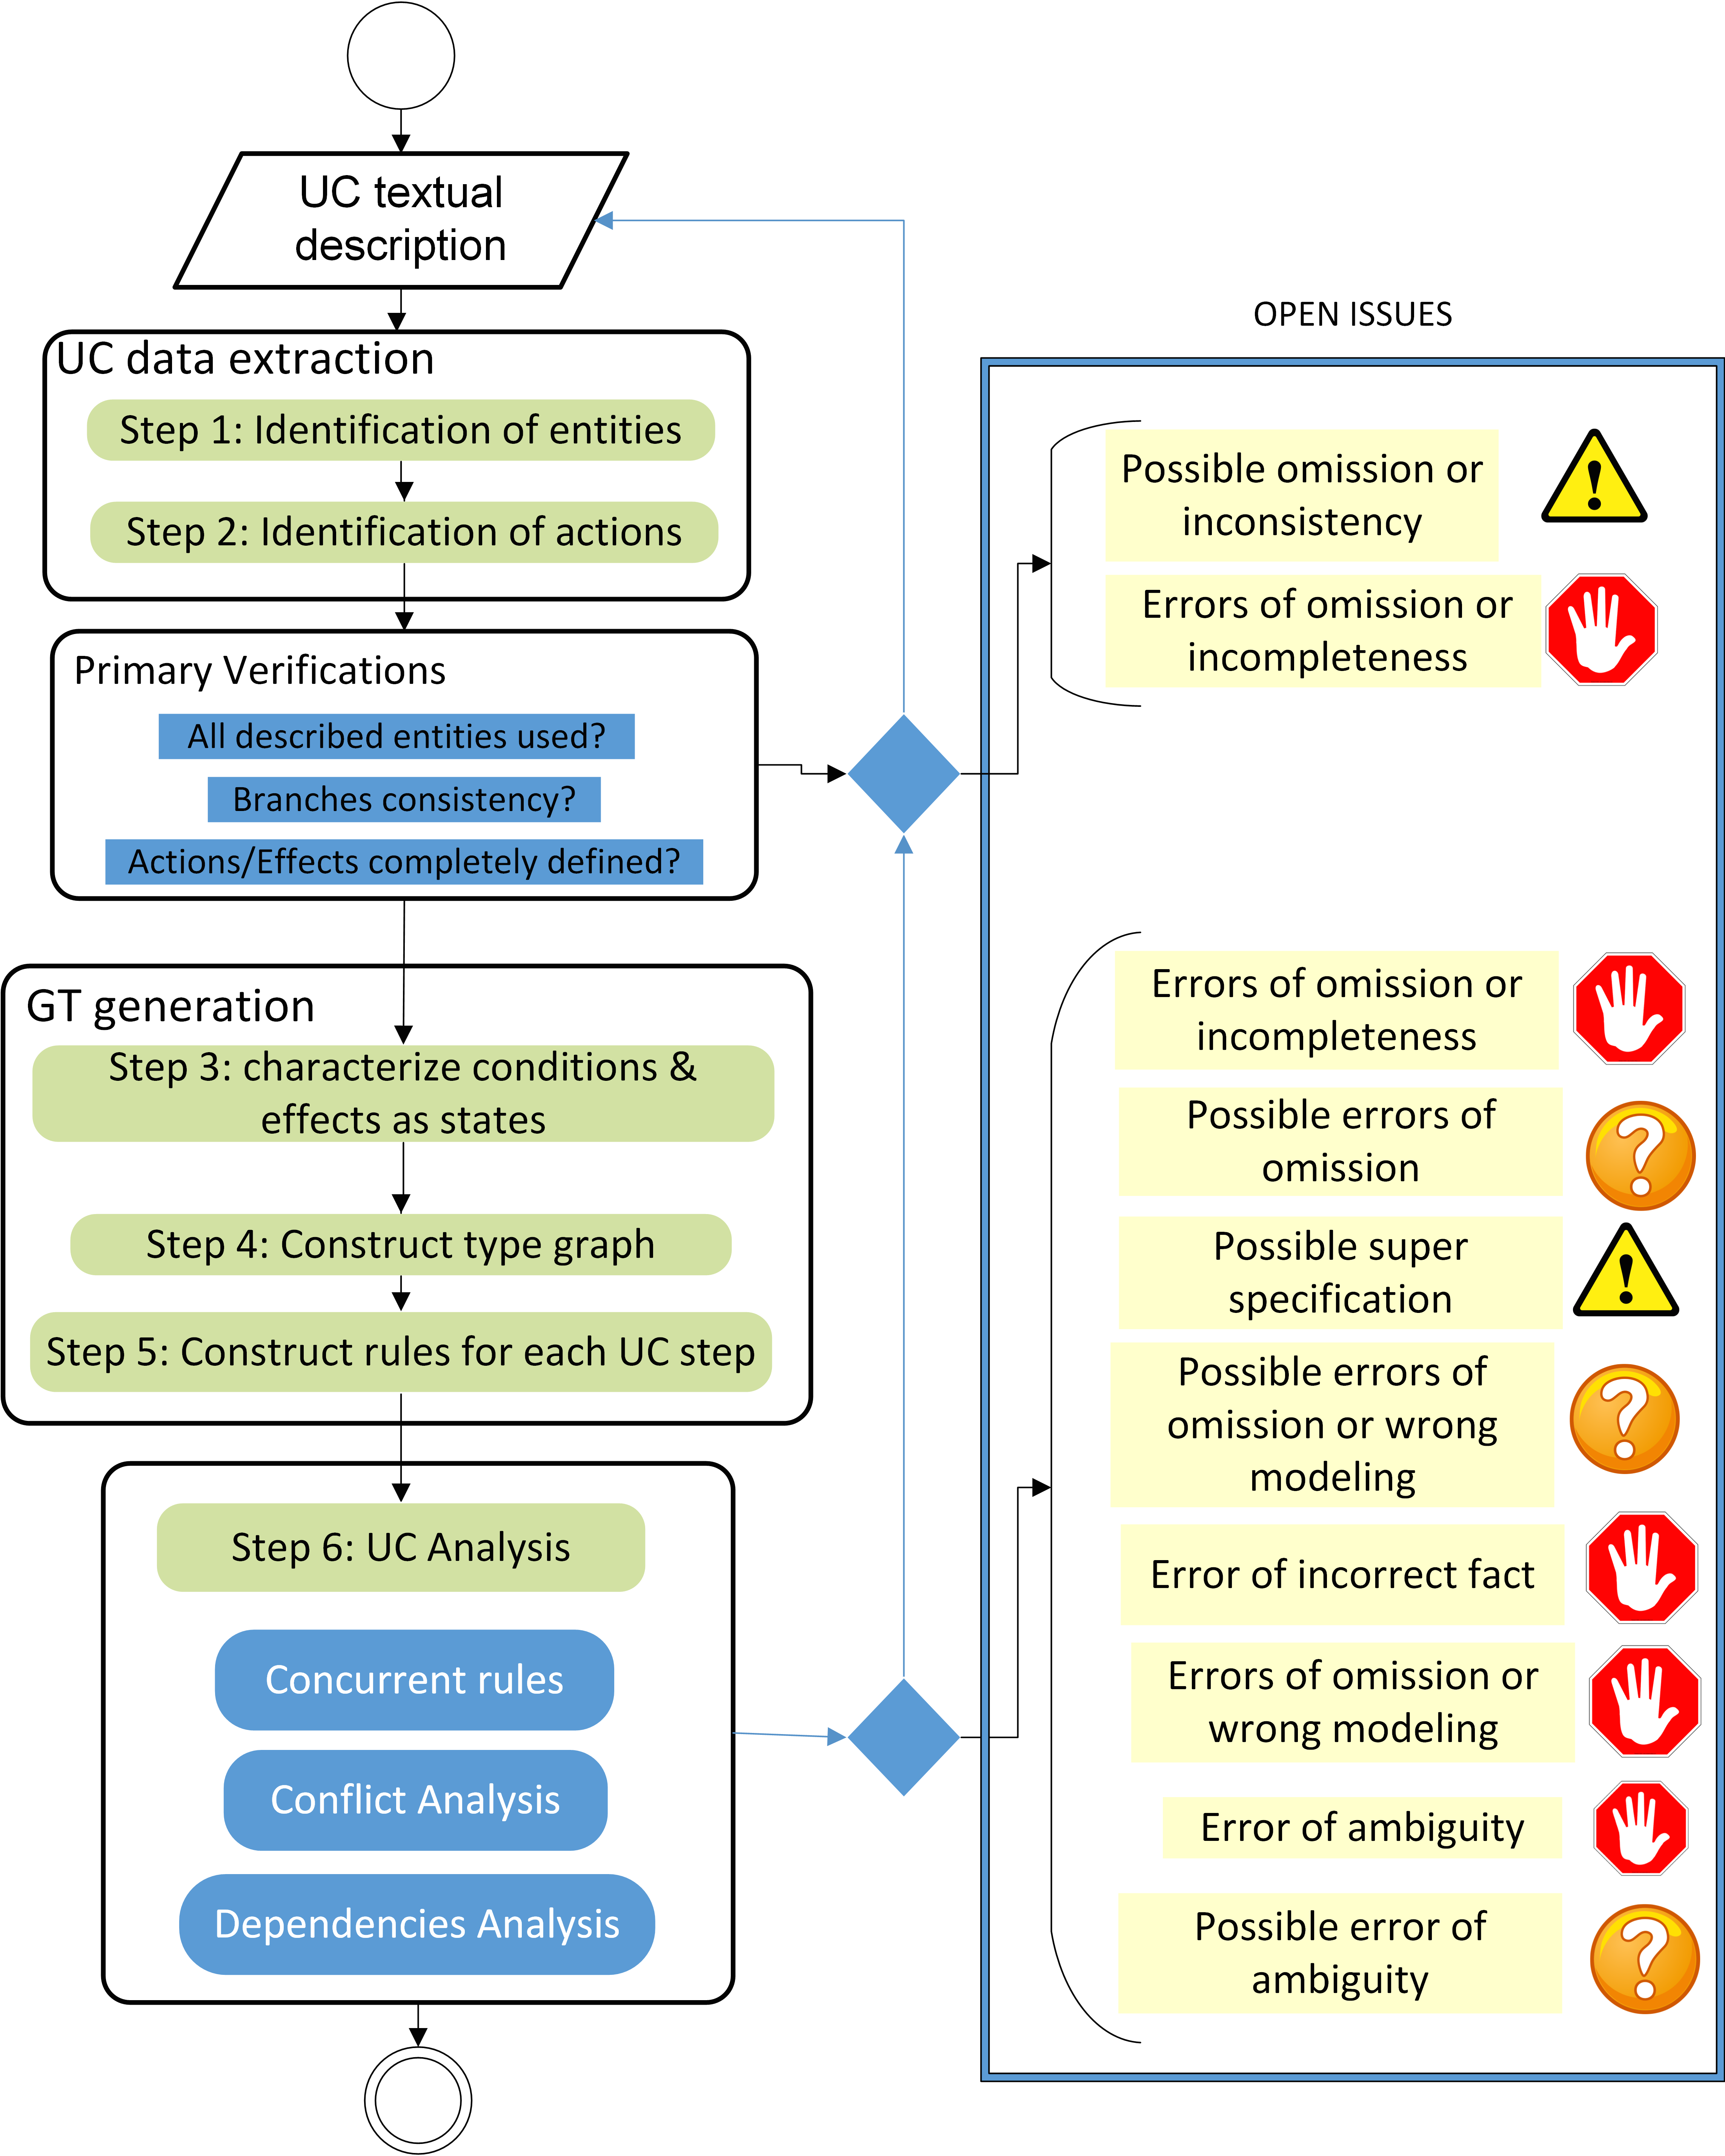
\includegraphics[scale=0.6]{images/generating-tests/methodology}}
  \caption{Overview of the methodology~\cite{Junior2015}.}\label{fig:tests:methodology}
\end{figure}

\section{Calculating tests using Occurrence Graph Grammars}

Given a graph grammar \graphGrammar{} modelling a system $X$ with $n > 0$ functionalities, we want to generate a test case for each subset of rules $F_i \subseteq P$ $\forall i \in 1\ldots n$, where $F_i$ represents a complete functionality \tinytodo{feature} of the system $X$.

Besides having the grammar $GG$ and knowing the subsets of functionalities $F_i$, we will also need an \emph{input-output relation} for each $F_i$ connecting the rules involved in the feature. This \emph{input-output relation} specifies which elements (nodes and edges) must be the same among the rules, as shown in example~\ref{ex:inout}.

Therefore, we want to know whether each functionality is executable. In the positive case, we want to know the input and output data necessary for this functionality, an ordering in which the rules can be applied in order to complete it, and which intermediary states can are valid. In the negative case, we want to know why this functionality can not be executed.

\begin{example}[Input-Output Relations]\label{ex:inout}
\end{example}

For the test cases generation we receive as input:

\begin{itemize}
\item set of rules $P$
\item subsets representing functionalities $F_i$
\item input-output relations $IO_i$ for each $F_i$
\end{itemize}

We want to generate as output:

\begin{itemize}
\item an amalgamation (colimit) $OGG_i$ of rules for each $F_i$ with respect to $IO_i$
\item the initial and final graphs $I_i$ and $J_i$ of $OGG_i$, representing the input and output data of the functionality $F_i$
\item the conflict and dependency relations between rules \tinytodo{and the elements involved in the conflict / dependency}
\item restrictions \tinytodo{remove or expand?}
\end{itemize}

\begin{example}[Amalgamation example]
\end{example}

\begin{example}[Initial and Final Graphs Example]
\end{example}

\begin{itemize}
  \item
  \item 
\end{itemize}

Once we have the output, we test whether $OGG_i$ is an occurrence graph grammar and $I_i, J_i$ are valid graphs.

\begin{example}[]
\end{example}

\section{Building test cases with Verigraph}

More specific usability details can be found on the Verigraph tutorial, whose current version is presented on appendix~\ref{app:tutorial}.\footnote{Tutorials for both older and newer releases of Verigraph are available at \url{https://github.com/Verites/verigraph/releases}.}
